\documentclass[screen]{beamer} % Se prefiere el tamaño screen para presentaciones.
\usetheme{Warsaw}
\usecolortheme{seahorse}
\setbeamercolor{title}{bg = cyan!50!black, fg= white}

\usepackage[utf8x]{inputenc}
\usepackage[spanish]{babel}
\spanishdatedel
\usepackage{graphicx,float,hyperref}

\title[Beamer]{Presentaciones con Beamer}
\author[Oromion]{Oromion}
\institute{Ubuntu Colombia}
\date{\today}
\begin{document}

\begin{frame}
\maketitle
\end{frame}

\begin{frame}{Contenido}
\tableofcontents % Solo aparecen secciones y subsecciones.
\end{frame}

%Es opcional que esté en el entorno frame.
\section{Una presentación simple}

\subsection{Comandos básicos de contenido}

\begin{frame}{\insertsubsection}{\insertsection}
\texttt{pause} es un comando de interacción
\pause
\begin{figure}[H]
\centering
\includegraphics[scale=0.5]{example-image-a}
\end{figure}
%Esta es una diapositiva.
%\write18{wget https://assets.ubuntu.com/v1/c037fd75-ubuntu-logo.png}
%
\includegraphics{c037fd75-ubuntu-logo.png}
\end{frame}

\subsection{Interrupciones}
\begin{frame}{\insertsubsection}{\insertsection}
\begin{enumerate}
\item<2-> Existencia de infinitos números primos.
%El número indica en qué diapositiva aparecerá.
\item<1-> Suponga $p$ un número muy grande.
Sea $q$ el producto de los primeros $p$.
\item<3-> Entonces $q+1$ no es divisible por ninguno de ellos.
\item<1-4> QED. %Desde la primera hasta la cuarta.
\end{enumerate}
\end{frame}

\begin{frame}
\begin{figure}[H]
\centering
\write18{wget http://www.jonathanleroux.org/software/iguanatex/iguana.jpg}
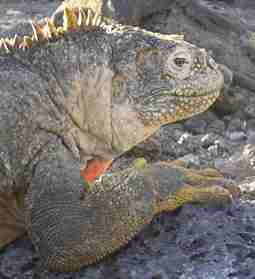
\includegraphics{iguana.jpg}
\end{figure}
\end{frame}
\end{document}
La última tarea es una presentación explicando uno de los temas del curso.